The assignment is about the logistic control of silicon wafers in an EUV ASML waferstepper. If a rack of wafers arrives at a EUV (Extreme Ultra Violet) waferstepper, they must enter the machine one by one via a sluice. There are two sluices, such that if one of the two sluices does not function the other can be used to let wafers enter and leave the machine.\\

There is one robot that picks wafers from the input rack and puts them in one of the two sluices. There is another robot inside the machine that takes wafers from the sluice and puts them into a waiting rack. A third robot moves the wafers from the waiting rack to the image projection system, and moves them back to another waiting rack after an image is projected. The wafers are subsequently moved outside the machine to an output rack.\\

It is prevented that the machine is out of production. So, under no circumstance it is allowed that a robot damages a door of a sluice, or the vacuum in the machine is destroyed because the two doors of a sluice are open at the same time. As wafers are extremely delicate, it is also not allowed to put two wafers on top of each other.\\

Unfortunately, the doors of the sluice are less reliable than the other parts of the machine, this means that they sometimes get stuck (due to the forces exerted on these doors by atmospheric pressure). If this happens, all wafers must enter and leave the system via a single sluice, and the controller must take care that this happens automatically, without unnecessary delay.

\begin{figure}[h]
    \centering
	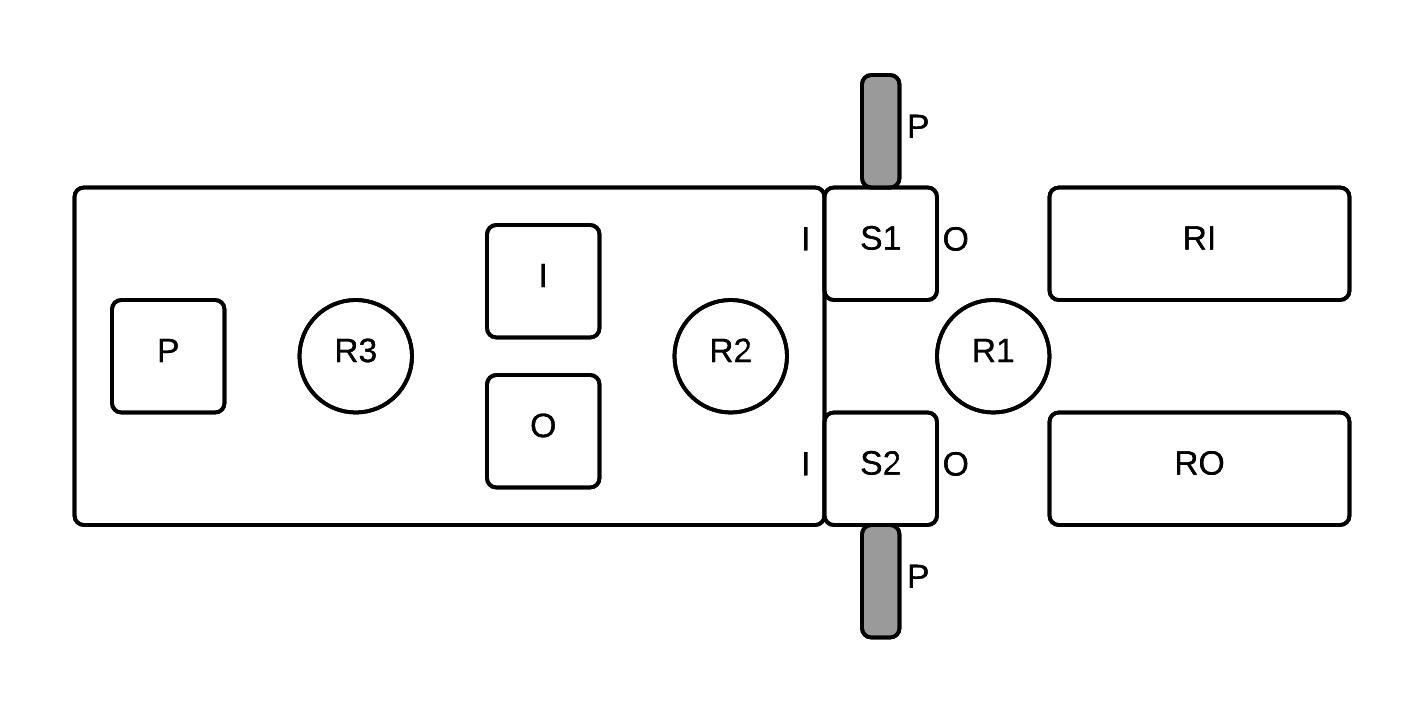
\includegraphics[width=0.7\textwidth]{waferstepper.png}
	\caption{\\P: Projector\\R3: Robot that places wafers under the projector\\I: Waiting rack for unprocessed wafers\\O: Waiting rack for processed wafers\\R2: Robot that moves wafers from sluices to the waiting racks and vice versa\\S1 and S2: Sluices, each sluice has an inside door I, an outside door O and a pump P\\R1: Robot that moves wafers from the input rack to the sluices and from the sluices to the output rack\\RI: Wafer input rack\\RO: Wafer output rack}
\end{figure}